\documentclass{bioinfo}
\copyrightyear{2020} \pubyear{2020}
\access{Advance Access Publication Date: Day Month Year}
\appnotes{Original Paper}

\begin{document}
\firstpage{1}

\subtitle{Structural bioinformatics}

\title[pyconsFold]{pyconsFold: Modelling and docking using distance contact predictions.}
\author{Lamb, J\,$^{\text{\sfb 1,2}}$, Elofsson, A\,$^{\text{\sfb 1,2}*}$}
\address{$^{\text{\sf 1}}$ Science for Life Laboratory, Stockholm University, SE-171 21 Solna, Sweden\\
$^{\text{\sf 2}}$Department of Biochemistry and Biophysics, Stockholm University, SE-106 91 Stockholm, Sweden}

\corresp{$^\ast$To whom correspondence should be addressed.}

\history{Received on XXXXX; revised on XXXXX; accepted on XXXXX}

\editor{Associate Editor: XXXXXXX}

\abstract{\textbf{Motivation:} Contact predictions within a protein has recently become a viable method for accurate prediction of protein structure. Using predicted distance distributions has been shown in many cases to be superior to only using a binary contact annotation. Using predicted inter protein distances has also been shown to be able to dock protein chains.\\ 
\textbf{Results:} Here we present pyconsFold. Using CNS as its underlying folding mechanism and predicted contact distance it outperforms regular contact prediction based modelling on our dataset of 210 proteins. It performs marginally lower than the state of the art pyRosetta folding pipeline but is on average about 20 times faster per model. pyconsFold also has a new novel way of using predicted inter protein contacts to simultaneously fold and dock two protein chains.\\
\textbf{Availability and implementation} pyconsFold is implemented in Python 3 with a strong focus on using as few dependencies as possible for longevity. It is available both as a pip package in Python 3 and as source code on \href{https://github.com/johnlamb/pyconsfold}{GitHub} and is published under the  GPLv3 license.\\
\textbf{Contact:} \href{arne@bioinfo.se}{arne@bioinfo.se}\\
\textbf{Supplementary information:} The full source code and documentation are available from \href{https://github}{https://github.com/johnlamb/pyconsfold}.}

\maketitle

\section{Introduction}
De novo protein modelling has recently seen significant improvements by relying on contact predictions that have been presented in binary format, two residues are either in contact (within 8Å) or not. By running mathematical models such as DCA on multiple seqeunce alignments we can extract possible contacts based on coevolutionary information and when these contacts are filtered using image recognition inspired deep learning we get good enough quality of the contacts to use for structure prediction. In the last few years we have again seen a significant improvement in structure prediction by using predicted distances between residues instead of just contacts(CASP13 \cite{Kryshtafovych2019-zb,Yang1496}). Historically, classifications has been easier to achieve (contact or not) in ,achine learning than regression but new advances, particularly in deep learning architecture, has now shown that these new methods can produce distances that results in better models than using just regular binary contacts.

CONFOLD\cite{Adhikari2015-fl} is a wrapper around CNS \cite{Brunger1998-ji,Brunger2007-ut} that uses predicted binary contacts together with predicted secondary structure to model proteins. pyconsFold is a re-implementation and extension of CONFOLD that achieves better results using distance predictions and that also expands to allow for more geometric restraints, such as angles predicted by tools such as trRosetta \cite{Yang1496}.

\section{Implementation}
pyconsFold is implemented in pyhon 3 as a wrapper around the CNS system used for folding proteins from NMR experimental data. It leverages CNS underlying power by converting predicted distances into geometric restraints. CNS ability to handle multiple chains are also leveraged to achieve the modelling and docking of complexes at the same time by using both inter and intra chain predicted contacts.\\
pyconsFold mainly runs in one stage as previous work \cite{Michel2017} has shown that running two stages only give marginal gains to the TM-score but more than doubles the run time.
pyconsFold has three major modes:

\subsection{Contact based modelling}
Contact based modelling or legacy modelling treats all contacts as binary contacts, they are in contact within 8Å. This mode can simulate CONFOLD by also including secondary structure prediction and setting the gaps parameter to 5, meaning only contacts separated by at least 5 residues will be used. In this mode it is most common to use a numbers threshold for how many contacts to use by the convetion of a multiple of protein length, eg 1.5L would mean to use 1.5 times the protein length number of contacts.

\subsection{Distance based modelling}
Distance based modelling works similar to classical modelling but in this case, an extra column is expected in the CASP-contacts file which defines the standard error for the predicted distance of the contact. By default this mode also includes contacts within 5 residues from each other and does not require a secondary structure file. Benchmark has even shown that this mode does not produce better models with a secondary structure file.

\subsection{Docking modelling}
Docking modelling uses CNSs underlying ability to model two protein chains simultaneously. A contact prediction file of both inter and intra contacts needs to be supplied. This can be achieved by running alignment tools for the two chains separately, concatenating these files horizontally and then treating this resulting alignment as one chain and using any contact prediction method to predict contacts. This contact file together with the original fasta files are used as inputs and models the full binary complex.

%\enlargethispage{12pt}
\begin{figure}%[!tpb]%figure1
  \centerline{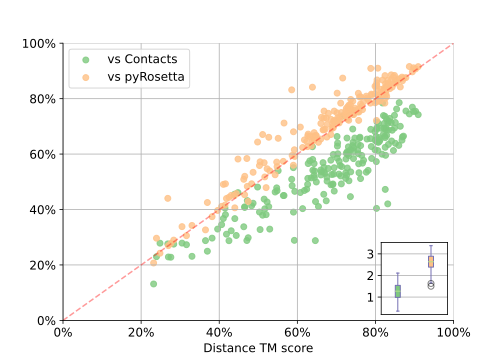
\includegraphics[width=\linewidth]{pyconsFold_figure}}
\caption{pyconsFold distance prediction against both contact base (green) and pyRosetta (orange) models. Distance predictions outperforms contact based predictions in almost all cases. pyconsFolds distance predicted models perform almost as well as pyRosetta but is around 20 times (more than 1 order of magnitude) faster per model as the inset shows(log10 scale of per model time in seconds. pyconsFold in green and pyRosetta in orange).}\label{fig:01}
\end{figure}

\section{Additional features}
For ease of use and reproducibility we have included several extra features and utilities. By default the generated models are ranked by CNS internal NOE energy but Quality Assessment score from pcons \cite{Lundstrom2008-wa} will also be calculated. If a native structure is known and supplied with the tmscore\_pdb\_file argument, the tmscore \cite{Zhang2007-xu,Xu2010-vu} for each model against the native structure will be calculated. 
Compiled versions of both pcons and TMscore for unix based x64 systems are packaged together with pyconsFold under the open source Boost license. If your system does not support the built in versions, you can manually install them on your system and as long as they are in your path, will be chosen instead of the built in binaries.

\section{Docking}

\section{Discussion}
pyconsFold offers a complete toolkit for ab initio modelling using predicted contact distances and angles. Its focus is on ease of use and reproducibility and is available both as source on github and as an easily installable pip package in Python 3. It comes packaged with QA-programs to rank the generated models and allows transparency for many tweakable parameters for the underlying CNS-system. It also offers a docking protocol where predicted inter chain contacts are used as restraints for docking. It offers a significant increase in accuracy over contact based protocols by using predicted distances. It is also around 20 times faster than pyRosetta per model.

%%%%%%%%%%%%%%%%%%%%%%%%%%%%%%%%%%%%%%%%%%%%%%%%%%%%%%%%%%%%%%%%%%%%%%%%%%%%%%%%%%%%%
%
%     please remove the " % " symbol from \centerline{\includegraphics{fig01.eps}}
%     as it may ignore the figures.
%
%%%%%%%%%%%%%%%%%%%%%%%%%%%%%%%%%%%%%%%%%%%%%%%%%%%%%%%%%%%%%%%%%%%%%%%%%%%%%%%%%%%%%%

\section*{Acknowledgements}
This work was supported by grants from 
the Swedish Research Council (VR-NT 2016-03798 to A.E.),
National Science Centre (No. 2012/07/E/NZ1/01900 to J.I.S. and
No. 2018/29/N/NZ2/02897 to A.I.J.).
\subsection*{Conflict of Interest Statement}
None delared.

% \bibliographystyle{unsrt}
\bibliographystyle{natbib}
%\bibliographystyle{achemnat}
%\bibliographystyle{plainnat}
%\bibliographystyle{abbrv}
%\bibliographystyle{bioinformatics}
%
%\bibliographystyle{plain}
%
\bibliography{references.bib}

\end{document}

